%
%  untitled
%
%  Created by andrea crotti on 2009-03-09.
%  Copyright (c) 2009 Andrea Crotti Corp. All rights reserved.
%
\documentclass[]{article}

% Use utf-8 encoding for foreign characters
\usepackage[utf8]{inputenc}

% Setup for fullpage use
\usepackage{fullpage}

% Uncomment some of the following if you use the features
%
% Running Headers and footers
%\usepackage{fancyhdr}

% Multipart figures
%\usepackage{subfigure}

% More symbols
%\usepackage{amsmath}
%\usepackage{amssymb}
%\usepackage{latexsym}

% Surround parts of graphics with box
\usepackage{boxedminipage}

% Package for including code in the document
\usepackage{listings}

% If you want to generate a toc for each chapter (use with book)
\usepackage{minitoc}

% This is now the recommended way for checking for PDFLaTeX:
\usepackage{ifpdf}

\ifpdf
\usepackage[pdftex]{graphicx}
\else
\usepackage{graphicx}
\fi
\title{Nomadic communication relation}
\author{Andrea Crotti, Fabio Cannioto, Alberto Scattolo, Christian Plattner}

\date{2009-03-09}

\begin{document}

\ifpdf
\DeclareGraphicsExtensions{.pdf, .jpg, .tif}
\else
\DeclareGraphicsExtensions{.eps, .jpg}
\fi

\maketitle
\lstset{numbers=left, numberstyle=\tiny, language=python}

\section{Intro}
% Describe what we are gonna do, the general ideas and what we are gonna talk about.
% Say what is needed to understand the sections that will follow.

The purpose of the project 
is the evaluation of the performances variation of a wireless network 802.11 b/g at the change of some parameters.
\\\newline
In order to make those tests we used some tools whitch are Iperf, wireshark, and a complex python script for the automated run test.
\\\newline
The test consist basicaly in many automatic execution of iperf with fixed time and different speed and finaly we consider the amount of transfering data.
\\\newline
The set of the tests was an indoor environment a notebook wich run iperf as server, an other notebook wich run iperf as client (throw the python script), a cisco ap and another notebook wich run wireshark to sniff the traffic.

\vspace{1cm}

\begin{figure}[h!]
	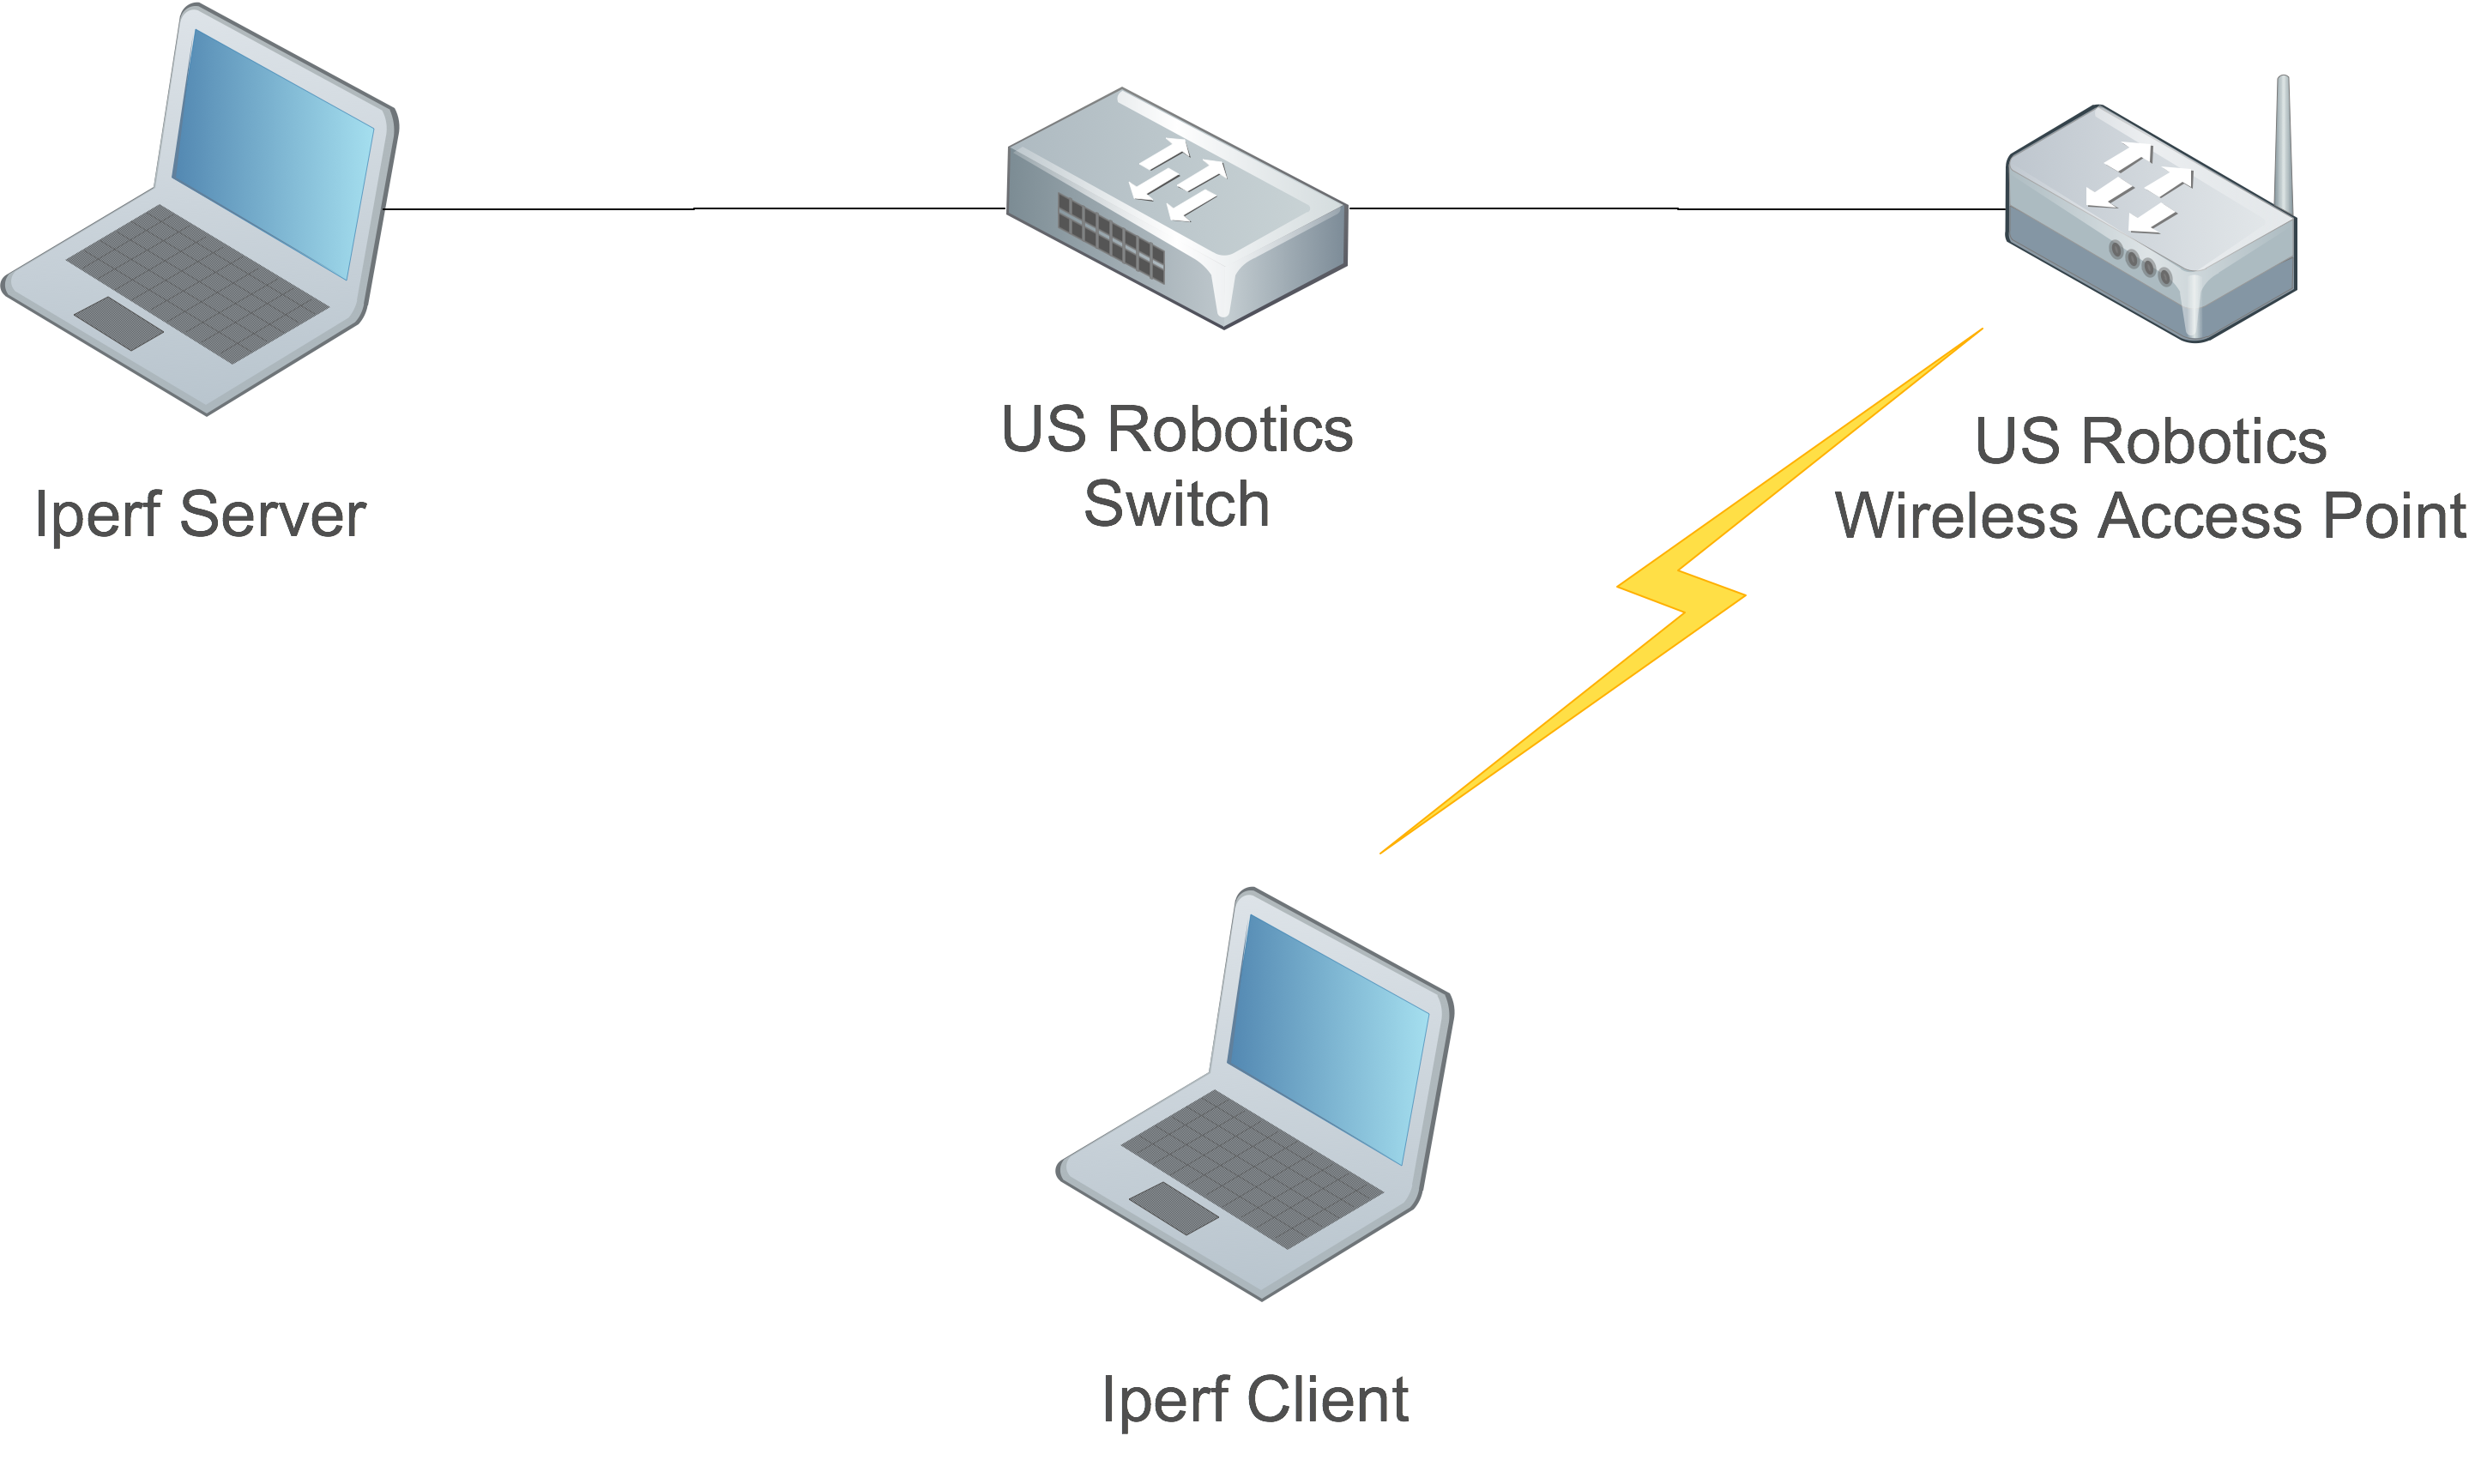
\includegraphics[angle=0, keepaspectratio=true, width=15cm]{images/network_overview}
	\caption{Network overview}
\end{figure}


\section{Software setup}
\subsection{Software} \label{setup:software}
	% ssh keys, iwconfig, python software, iperf, tcpdump, gnuplot, whatever used


\bibliographystyle{plain}
\bibliography{}
\end{document}
